\section{Подобие многоугольников}

\paragraph{}\label{1938/168}
\so{Определение}.
Два $n$-угольника называются \rindex{подобные!многоугольники}\textbf{подобными}, если углы одного равны соответственно углам другого и соответственные стороны пропорциональны.

Во избежании путаницы у подобных многоугольников принято записывать соответственные вершины в том же порядке.
Например «пятиугольник
$ABCDE$ подобен пятиугольнику $A_1B_1C_1D_1E_1$» (рис.~\ref{1938/ris-180}) обычно означает, что  
\[\angle A = \angle A_1, 
\quad
\angle B=\angle B_1,
\quad
\angle C=\angle C_1,
\quad
\angle D=\angle D_1,
\quad
\angle E=\angle E_1\]
и
\[\frac{AB}{A_1B_1}=\frac{BC}{B_1C_1}=\frac{CD}{C_1D_1}=\frac{DE}{D_1E_1}=\frac{EA}{E_1A_1}\]
При этом пары сторон $AB$ и $A_1B_1$, $BC$ и $B_1C_1$, $CD$ и $C_1D_1$, $DE$ и $D_1E_1$, $AE$ и $A_1E_1$
являются соответственными.

То, что такие многоугольники существуют, будет видно из решения следующей задачи:

\paragraph{}\label{1938/169}
\so{Задача}.
\emph{Дан многоугольник $ABCDE$ и отрезок $a$.
Построить другой многоугольник, который был бы подобен данному и у которого сторона, соответственная стороне $AB$ 
равнялась бы $a$} (рис.~\ref{1938/ris-179}).

\begin{figure}[h]
\centering
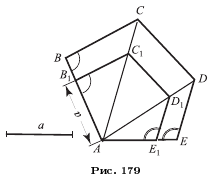
\includegraphics{mppics/ris-179}
\caption{}\label{1938/ris-179}
\end{figure}

На стороне $AB$ отложим $AB_1=a$ (если $a>AB$, то точка $B_1$ расположится на продолжении $AB$).
Затем, проведя из $A$ все диагонали, построим $B_1C_1 \parallel BC$, $C_1D_1\parallel CD$ и $D_1E_1\parallel DE$.

Тогда получим многоугольник $AB_1C_1D_1E_1$, подобный многоугольнику $ABCDE$.
Действительно, во-первых, углы одного из них соответственно равны углам другого;
так, угол $A$ у них общий, $\angle B_1=\angle B$ и $\angle E_1=\angle E$ как соответственные углы при параллельных прямых;
$\angle C_1=\angle C$ и $\angle D_1=\angle D$, так как углы эти состоят из частей, соответственно равных друг другу.

Во-вторых, мы имеем пропорции:
\begin{align*}
\text{из подобия }&\ \triangle AB_1C_1\sim\triangle ABC:
&
\frac{AB_1}{AB}=\frac{B_1C_1}{BC}=\frac{AC_1}{AC};
\\
\text{—\textquotedbl—\textquotedbl—\quad}&\ \triangle AC_1D_1\sim\triangle ACD:
&
\frac{AC_1}{AC}=\frac{C_1D_1}{CD}=\frac{AD_1}{AD};
\\
\text{—\textquotedbl—\textquotedbl—\quad}&\ \triangle AD_1E_1\sim\triangle ADE:
&
\frac{AD_1}{AD}=\frac{D_1E_1}{DE}=\frac{AE_1}{AE}.
\end{align*}

Так как третье отношение первого ряда равно первому отношению второго ряда и третье отношение второго ряда равно первому отношению третьего ряда, то значит, все 9 отношений равны между собой.
Выбросив из них отношения, в которые входят диагонали, можем написать:
\[\frac{AB_1}{AB}=\frac{B_1C_1}{BC}=\frac{C_1D_1}{CD}=\frac{D_1E_1}{DE}=\frac{AE_1}{AE}.\]

Мы видим, что у $n$-угольников $ABCDE$ и $AB_1C_1D_1E_1$ соответственные углы  равны и соответственные стороны пропорциональны;
значит, многоугольники эти подобны.

{\small

\paragraph{}\label{1938/170}
\so{Замечание}.
Для треугольников, как мы видели (§~\ref{1938/161}), равенство углов влечёт пропорциональность сторон, и обратно:
пропорциональность сторон влечёт равенство углов;
вследствие этого для треугольников одно равенство углов или одна пропорциональность сторон служит достаточным признаком их подобия.
Для многоугольников же одного равенства углов или одной пропорциональности сторон ещё недостаточно для их подобия:
например, у квадрата и прямоугольника углы равны, но стороны не пропорциональны, у квадрата же и ромба стороны пропорциональны, а углы не равны.

}

\paragraph{}\label{1938/171}
\so{Теорема} (о разложении подобных многоугольников на подобные треугольники).
\textbf{\emph{Подобные многоугольники можно разложить на одинаковое число подобных и одинаково расположенных треугольников.}}

Например, подобные многоугольники $ABCDE$ и $AB_1C_1D_1E_1$ (рис. \ref{1938/ris-179}) разделены диагоналями на подобные треугольники, которые одинаково расположены — если пара треугольников в $ABCDE$ имеет общую сторону, то тоже верно и про пару им сходственных треугольников в $AB_1C_1D_1E_1$ и наоборот.


Укажем ещё такой способ разложения.
Возьмём внутри многоугольника $ABCDE$ (рис.~\ref{1938/ris-180}) произвольную точку $O$ и соединим её со всеми вершинами.
Тогда многоугольник $ABCDE$ разобьётся на столько треугольников, сколько в нём сторон.
Возьмём один из них, например $AOE$ (покрытый на рисунке штрихами), и на соответственной стороне $A_1E_1$ другого многоугольника построим углы $O_1A_1E_1$ и $O_1E_1A_1$ соответственно равные углам $OAE$ и $OEA$;
точку пересечения $O_1$ соединим с прочими вершинами многоугольника $A_1B_1C_1D_1E_1$.
Тогда и этот многоугольник разобьётся на то же число треугольников.
Докажем, что треугольники первого многоугольника соответственно подобны треугольникам второго многоугольника.

По построению $\triangle AOE\sim \triangle A_1O_1E_1$. 
Чтобы доказать подобие соседних треугольников $ABO$ и $A_1B_1O_1$, примем во внимание, что из подобия многоугольников следует:
\[\angle BAE=\angle B_1A_1E_1
\quad\text{и}\quad
\frac{BA}{B_1A_1}=\frac{AE}{A_1E_1},
\eqno(1)\]
и из подобия треугольников $AOE$ и $A_1O_1E_1$ выводим:
\[\angle OAE=\angle O_1A_1E_1
\quad\text{и}\quad
\frac{AO}{A_1O_1}=\frac{AE}{A_1E_1}.
\eqno(2)\]
Из равенств (1) и (2) следует:
\[\angle BAO=\angle B_1A_1O_1
\quad\text{и}\quad
\frac{BA}{B_1A_1}=\frac{AO}{A_1O_1}.\]
Теперь видим, что треугольники $ABO$ и $A_1B_1O_1$ имеют по равному углу, заключённому между пропорциональными сторонами;
значит, они подобны.

Совершенно так же докажем, что подобие $\triangle BCO\sim \triangle B_1C_1O_1$, затем $\triangle CDO\sim\triangle C_1D_1O_1$, и~т.~д.
При этом заметим, треугольники первого многоугольника располагаются одинаково с подобными им треугольниками второго многоугольника. % изменена фраза

\begin{figure}[h]
\centering
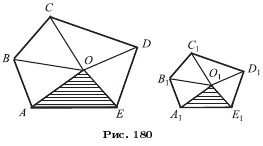
\includegraphics{mppics/ris-180}
\caption{}\label{1938/ris-180}
\end{figure}

\paragraph{}\label{1938/172}
\so{Теорема}.
\textbf{\emph{Периметры подобных многоугольников относятся как соответственные стороны.}}

Пусть многоугольники $ABCDE$ и $A_1B_1C_1D_1E_1$ (рис.~\ref{1938/ris-180}) подобны;
тогда по определению: 
\[\frac{AB}{A_1B_1}=\frac{BC}{B_1C_1}=\frac{CD}{C_1D_1}=\frac{DE}{D_1E_1}=\frac{EA}{E_1A_1}.\]
Если имеем ряд равных отношений, то сумма всех предыдущих членов относится к сумме всех последующих, как какой-нибудь из предыдущих членов относится к своему последующему, поэтому
\[\frac{AB+BC+CD+DE+EA}{A_1B_1+B_1C_1+C_1D_1+D_1E_1+E_1A_1}=\frac{AB}{A_1B_1}=\frac{BC}{B_1C_1}=\dots\]


\paragraph{Коэффициент подобия.}\label{1938/173}
Отношение соответственных сторон двух подобных многоугольников (в частности  треугольников) называется \rindex{коэффициент подобия}\textbf{коэффициентом подобия} этих многоугольников.

\paragraph{Центрально-подобное преобразование.}\label{1938/174}
Способ построения многоугольника, подобного данному, изложенный в §~\ref{1938/169}, является частным видом так называемого центрально-подобного преобразования.

\begin{wrapfigure}{o}{56mm}
\centering
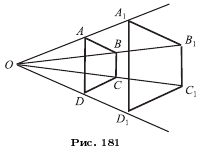
\includegraphics{mppics/ris-181}
\caption{}\label{1938/ris-181}
\end{wrapfigure}

Общий метод такого преобразования состоит в следующем.
Пусть требуется подобно преобразовать четырёхугольник $ABCD$ (рис.~\ref{1938/ris-181}) при коэффициенте подобия, равном $k$.
Возьмём какую-нибудь точку $O$ на плоскости;
соединив её с вершинами данного четырёхугольника, получим прямые $OA$, $OB$, $OC$ и $OD$.
На прямой $OA$ отложим от точки $O$ в сторону точки $A$ отрезок $OA_1$, равный $k\cdot OA$, так что $OA_1=k\cdot OA$ (на рисунке $k=\tfrac53$).

Продолжим также прямую $OB$ и отложим на ней от точки $O$ в сторону точки $B$ отрезок $OB_1$, равный $k\cdot OB$, так что $OB_1=k\cdot OB$.

Точно так же поступим с прямыми $OC$ и $OD$.
Мы получим на них точки $C_1$ и $D_1$, причём $OC_1=k\cdot OC$ и $OD_1=k\cdot OD$.
Соединив последовательно точки $A_1$, $B_1$, $C_1$ и $D_1$, получим искомый четырёхугольник $A_1B_1C_1D_1$.
В самом деле, из равенств $OA_1=k\cdot OA$, $OB_1=k\cdot OB$, $OC_1=k\cdot OC$ и $OD_1=k\cdot OD$ следует:
\[\frac{OA_1}{OA}=
\frac{OB_1}{OB}=
\frac{OC_1}{OC}=
\frac{OD_1}{OD}=k.\]

Сравним треугольники $OAB$ и $OA_1B_1$.
Они имеют общий угол в вершине $O$ и, кроме того,
\[\frac{OA_1}{OA}=
\frac{OB_1}{OB},\]
следовательно, эти треугольники подобны (§~\ref{1938/161}, 2-й случай).
Из их подобия заключаем:
\[\frac{A_1B_1}{AB}=
\frac{OA_1}{OA}=k
\quad\text{и}\quad
\angle OAB=\angle OA_1B_1,
\eqno(1)
\]
следовательно, $AB\parallel A_1B_1$ (§~\ref{1938/73}).

Совершенно так же покажем, что треугольники $OBC$ и $OB_1C_1$ подобны.
Отсюда следует:
\[\frac{B_1C_1}{BC}=
\frac{OB_1}{OB}=k
\quad\text{и}\quad
\angle OBC=\angle OB_1C_1,
\eqno(2)
\]
и, следовательно, $BC\parallel B_1C_1$.

Таким же образом докажем подобие следующих треугольников:
$OCD$ и $OC_1D_1$, затем треугольников $OAD$ и $OA_1D_1$.

Из подобия $\triangle OCD$ и $\triangle OC_1D_1$ следует:
\[\frac{C_1D_1}{CD}=
\frac{OC_1}{OC}=k
\quad\text{и}\quad
CD\parallel C_1D_1,
\eqno(3)
\]

Из подобия $\triangle OAD$ и $\triangle OA_1D_1$ следует:
\[\frac{A_1D_1}{AD}=
\frac{OD_1}{OD}=k
\quad\text{и}\quad
AD\parallel A_1D_1,
\eqno(4)
\]
Кроме того, $\angle DAB=\angle D_1A_1B_1$ как углы с параллельными сторонами (§~\ref{1938/79}).

По той же причине имеем равенство углов.
\begin{align*}
\angle ABC &= \angle A_1B_1C_1,
\\
\angle BCD &= \angle B_1C_1D_1,
\\
\angle CDA &= \angle C_1D_1A_1.
\end{align*}
Мы видим, что у четырёхугольников $ABCD$ и $A_1B_1C_1D_1$ соответственные углы равны и соответственные стороны пропорциональны;
значит, эти четырёхугольники подобны, причём коэффициент их подобия равен $k$.

\paragraph{Центр подобия.}\label{1938/175}\rindex{центр!подобия}
При центрально-подобном преобразовании многоугольника способом, изложенным в §~\ref{1938/174}, точка $O$ называется центром подобия обоих многоугольников.

Центрально-подобное преобразование многоугольника можно выполнять несколько иначе.
Именно, взяв точку $O$ и соединив её с вершинами четырёхугольника $ABCD$, можно продолжить прямые $OA$, $OB,\dots$
за точку $O$;
затем на прямой $OA$ от точки $O$ в сторону, противоположную точке $A$, отложим отрезок $OA'$, равный $k\cdot OA$.
Точно так же на продолжениях прямых $OB$, $OC,\dots$
от точки $O$ отложим отрезки $OB', OC',\dots$, равные соответственно отрезкам $k\cdot OB, k\cdot OC,\dots$
(рис.~\ref{1938/ris-182});
соединив последовательно точки $A'$, $B'$, $C'$, $D'$ получим четырёхугольник $A'B'C'D'$, очевидно симметричный с $A_1B_1C_1D_1$ относительно точки $O$.
Следовательно, четырёхугольники $A'B'C'D'$ и $A_1B_1C_1D_1$ равны и, значит, четырёхугольники $ABCD$ и $A'B'C'D'$ подобны, причём коэффициент их подобия равен $k$.
При первом способе преобразования точка $O$ называется {}\textbf{внешним центром} подобия многоугольников (рис.~\ref{1938/ris-181});
при втором способе — \rindex{центр!подобия}\textbf{внутренним центром} их подобия (рис.~\ref{1938/ris-182}).

\begin{figure}[h]
\centering
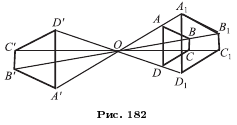
\includegraphics{mppics/ris-182}
\caption{}\label{1938/ris-182}
\end{figure}

{\small

\smallskip
\so{Замечание}.
При выполнении центрально-подобного преобразования можно одинаково пользоваться как внутренним, так и внешним центром подобия.
И тот и другой можно выбирать совершенно произвольно, в частности, если принять одну из вершин многоугольника за внешний центр подобия и выполнить центрально-подобное преобразование, то получим как раз тот способ построения подобного многоугольника, который был изложен в §~\ref{1938/169}.

}

\paragraph{Центрально-подобное расположение многоугольников.}\label{1938/176}
Расположение двух многоугольников $ABCD$ и $A_1B_1C_1D_1$ на рис.~\ref{1938/ris-181}, а также многоугольников $ABCD$ и $A'B'C'D'$ на рис.~\ref{1938/ris-182} имеет следующие свойства:
1) соответственные стороны обоих многоугольников параллельны;
2) прямые, соединяющие соответственные вершины, пересекаются в одной точке.

\begin{figure}[h]
\centering
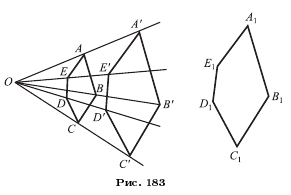
\includegraphics{mppics/ris-183}
\caption{}\label{1938/ris-183}
\end{figure}

{\sloppy 
Такое расположение многоугольников называется центрально-подобным. 
Докажем, что в такое расположение можно привести любые два подобных многоугольника.

}

Пусть даны два подобных многоугольника $ABCDE$ и $A_1B_1C_1D_1E_1$ (рис.~\ref{1938/ris-183}).
Возьмём какую-либо точку $O$ за центр подобия и построим многоугольник, центрально-подобный  с $ABCDE$, причём коэффициент подобия возьмём равным отношению $\frac{A_1B_1}{AB}$.
Мы получим многоугольник $A'B'C'D'E'$, подобный $ABCDE$ и в то же время равный $A_1B_1C_1D_1E_1$.
В самом деле, так как коэффициент подобия многоугольников $ABCDE$ и $A'B'C'D'E'$ равен $\frac{A_1B_1}{AB}$, то $\frac{A'B'}{AB}=\frac{A_1B_1}{AB}$, отсюда $A'B'=A_1B_1$.
Но многоугольники $A_1B_1C_1D_1E_1$ и $A'B'C'D'E'$ подобны между собой, следовательно:
\[\frac{A'B'}{A_1B_1}=\frac{B'C'}{B_1C_1}=\frac{C'D'}{C_1D_1}=\frac{D'E'}{D_1E_1}=\frac{A'E'}{A_1E_1}.\]
А потому из равенства $A'B'=A_1B_1$ вытекает 
\begin{align*}
B'C'&=B_1C_1,&
C'D'&=C_1D_1,&
D'E'&=D_1E_1,&
A'E'&=A_1E_1.
\end{align*}
Так как, кроме того, углы многоугольника $A_1B_1C_1D_1E_1$ равны соответствующим углам многоугольника $A'B'C'D'E'$, то эти многоугольники равны между собой. 
Если наложить многоугольник $A_1B_1C_1D_1E_1$ на  $A'B'C'D'E'$ так, чтобы они совпадали, то многоугольник $A_1B_1C_1D_1E_1$ примет центрально-подобное расположение с $ABCDE$. 

В случае если $k=1$ то многоугольники равны.
В этом случае следует взять $O$ как внутренний центр подобия, иначе многоугольник $A'B'C'D'E'$ сольётся с $ABCDE$.

\section{Подобие произвольных фигур}

\paragraph{}\label{1938/177}
{\sloppy 
Центрально-подобное преобразование многоугольников даёт возможность обобщить само понятие о подобии на случай, когда фигура образована кривыми линиями.
Именно такой способ построения подобной фигуры можно применить к любой фигуре.
Пусть, например, на плоскости дана фигура $A$ совершенно произвольной формы (рис.~\ref{1938/ris-184}).

}

\begin{figure}[h]
\centering
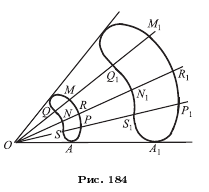
\includegraphics{mppics/ris-184}
\caption{}\label{1938/ris-184}
\end{figure}

Возьмём произвольную точку $O$ на плоскости этой фигуры и будем соединять её с различными точками $M$, $N$, $P,\dots$
фигуры $A$.
На каждой из проведённых прямых $OM$, $ON$, $OP,\dots$
отложим отрезки $OM_1$, $ON_1$, $OP_1$, такие, что 
\[\frac{OM_1}{OM}=\frac{ON_1}{ON}=\frac{OP_1}{OP}=\dots\quad\text{и так далее}\]
Точки $M_1$, $N_1$, $P_1,\dots$ будут лежать на некоторой новой фигуре $A_1$.
Чем больше точек $M$, $N$, $P,\dots$
мы возьмём на фигуре $A$, тем больше мы получим точек фигуры $A_1$.
Чтобы получить всю фигуру $A_1$, нужно провести прямые из точки $O$ ко всем точкам фигуры $A$ и построить на них соответствующие точки фигуры $A_1$.
Считается, что фигуры $A_1$ и $A$ расположены центально-подобно,
а любая фигура равная $A_1$ считается подобной~$A$.

В отдельных случаях, чтобы получить фигуру $A_1$, нет необходимости проводить лучи ко всем точкам фигуры $A$, достаточно построить лишь несколько её точек, и затем, пользуясь частными свойствами фигуры $A$, восстановить всю фигуру $A_1$.
Так, в том случае, когда $A$ — многоугольник, достаточно было соединить точку $O$ лишь с вершинами этого многоугольника и построить вершины подобного многоугольника, а затем соединить прямолинейными отрезками полученные вершины между собой.

{\sloppy 
Описанный переход от фигуры $A$ к фигуре $A_1$ называется \rindex{центрально-подобное преобразование}\textbf{центрально-подобным преобразованием}. 
Этот тип преобразований имеет заметное применение на практике.
Показываемая в кино картина на экране подобна изображению, сделанному на плёнке;
технические чертежи планов и фасадов зданий, планов местности, планов городов
получаются в результате подобного преобразования.

}

{\sloppy

\paragraph{Подобие окружностей.}\label{1938/178}
Докажем, что фигура, подобная окружности, есть также окружность.

}

\smallskip

\so{Теорема}.
\textbf{\emph{Геометрическое место точек, делящих в данном отношении отрезки, соединяющие какую-нибудь точку с точками окружности, есть окружность.}}


\begin{figure}[h]
\centering
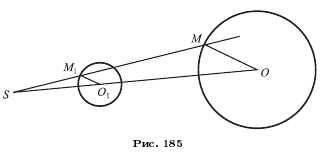
\includegraphics{mppics/ris-185}
\caption{}\label{1938/ris-185}
\end{figure}

Пусть дана окружность радиуса $R$ с центром в точке $O$ (рис.~\ref{1938/ris-185}).
Возьмём произвольную точку $S$ и, соединив её с точкой $O$, разделим отрезок $SO$ точкой $O_1$ в некотором отношении так, что $\frac{SO_1}{SO}= k$.

Возьмём произвольную точку $M$ на данной окружности и соединим её с точкой $S$.
На отрезке $SM$ найдём точку $M_1$ такую, что $\frac{SM_1}{SM}\z=\frac{SO_1}{SO}= k$.
Для этой цели следует из точки $O_1$ провести прямую, параллельную $OM$, до пересечения с прямой $SM$.
Из подобия треугольников $SOM$ и $SO_1M_1$.
следует $\frac{OM_1}{OM}=\frac{SO_1}{SO}$.
Следовательно, $\frac{OM_1}{OM}=k$.
Отсюда найдём длину отрезка $O_1M_1$, именно $O_1M_1=k\cdot OM$, или $O_1M_1=k\cdot R$.

Мы видим, что величина $O_1M_1$ не зависит от положения точки $M$ на данной окружности.
Следовательно, если точка $M$ будет перемещаться по окружности, то точка $M$\ будет перемещаться по плоскости, описывая окружность с центром $O_1$ и радиусом~$k\cdot R$.

\paragraph{}\label{1938/179}
\so{Теорема}.
\textbf{\emph{Две окружности на плоскости всегда можно рассматривать как центрально-подобные фигуры, причём окружности разных радиусов имеют два центра подобия:
один внешний, другой внутренний.}} 

Пусть даны две окружности с центрами $O_1$ и $O_2$ и радиусами $R_1$ и $R_2$ (рис.~\ref{1938/ris-186}).
Проведём линию центров $O_1O_2$ и построим на ней две точки $I$ и $E$, определяемые равенствами
\[\frac{O_1I}{O_2I}=\frac{R_1}{R_2}\quad\text{и}\quad\frac{O_1E}{O_2E}=\frac{R_1}{R_2}\]
(Точка $I$ на отрезке $O_1O_2$ существует всегда, а точка $E$ на продолжении отрезка существует только если $R_1\ne R_2$.)

Покажем, что точки $I$ и $E$ обладают свойствами центров подобия.
Возьмём какую-либо точку $M_1$ на первой окружности, проведём прямую $IM_1$ и отложим на ней отрезок $IM_2$ так, что 
\[\frac{IM_1}{IM_2}=\frac{R_1}{R_2}.\] 
Тогда $\triangle IO_1M_1\sim\triangle IO_2M_2$, так как 
\begin{align*}
\angle O_1IM_1&=\angle O_2IM_2,
\\
\frac{IM_1}{IM_2}&=\frac{R_1}{R_2},
\\
\frac{O_1I}{O_2I}&=\frac{R_1}{R_2}.
\end{align*}
Следовательно:
\[\frac{O_1M_1}{O_2M_2}=\frac{R_1}{R_2},\]
и, так как $O_1M_1=R_1$, поучаем
\[O_2M_2=R_2.\]
Это означает, что точка $M_2$ лежит на второй окружности.
Следовательно, точка $I$ есть внутренний центр подобия данных окружностей.
Таким же образом можно доказать, что $E$ есть внешний центр подобия.

\begin{figure}[h]
\centering
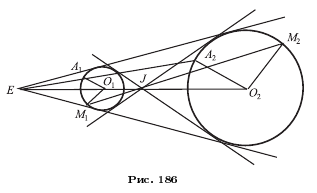
\includegraphics{mppics/ris-186}
\caption{}\label{1938/ris-186}
\end{figure}

Построение точек $I$ и $E$ можно выполнить так:
проводим в данных окружностях два каких-либо параллельных радиуса и соединяем их концы, полученная прямая пересечёт линию центров в центре подобия.
При этом если проведённые радиусы направлены в одну сторону (рис.~\ref{1938/ris-186}, $O_1A_1$, и $O_2A_2$), то центр подобия будет внешним;
если они направлены в противоположные стороны (рис.~\ref{1938/ris-186}, $O_1M_1$ и $O_2M_2$), то центр подобия будет внутренним.
В случае равенства $R_1=R_2$ вторая прямая будет параллельна линии центров, в этом случае нет внешнего центра $E$.

\smallskip

Легко далее заметить, что если две окружности касаются, то один из центров подобия совпадает с точкой касания.
При этом если касание окружностей внешнее, то в точке касания находится внутренний центр подобия, если же касание внутреннее, то с точкой касания совпадает внешний центр подобия окружностей.

\smallskip
\so{Упражнения 1}.
Доказать, что если две окружности лежат одна вне другой, то их внешний центр подобия совпадает с точкой пересечения их общих внешних касательных, а внутренний — с точкой пересечения общих внутренних касательных.

2.
Какое положение должны иметь две окружности на плоскости, чтобы их внешний центр подобия совпал с внутренним? 

\smallskip
\so{Ответ}.
Окружности концентричны.


\subsection*{Задачи на построение}

\paragraph{Метод подобия.}\label{1938/181}
Центрально-подобное преобразование фигур можно с успехом применить к решению многих задач на построение.
На этом основан так называемый метод подобия.

Метод подобия состоит в том, что, пользуясь некоторыми данными задачи, строят сначала фигуру, \so{подобную} искомой, а затем переходят к искомой.
Этот метод особенно удобен тогда, когда только одна данная величина есть длина, а все прочие величины — или углы, или отношения линий;
таковы, например, задачи:
построить треугольник по данному углу, стороне и отношению двух других сторон или по двум углам и длине некоторого отрезка (например высоте, медиане или биссектрисе);
построить квадрат по данной сумме или разности между диагональю и стороной.

Решим, например, такую задачу:

\smallskip
\so{Задача 1}.
\emph{Построить треугольник, когда даны один из его углов $C$, отношение сторон $AC:BC$, заключающих этот угол, и высота $h$, опущенная из вершины этого угла на противоположную сторону} (рис.~189).

Пусть $AC:BC=m:n$, где $m$ и $n$ — два данных отрезка или два данных числа.
Строим угол $C$, на его сторонах откладываем отрезки $CA_1$ и $CB_1$, пропорциональные $m$ и $n$.
Если $m$ и $n$ — отрезки, то берём прямую $CA_1=m$ и $CB_1=n$.
Если $m$ и $n$ — числа, то, выбрав произвольный отрезок $\ell$, строим отрезки $CA_1\z=m \cdot \ell$, и $CB_1=n\cdot \ell$.
В обоих случаях имеем
\[\frac{CA_1}{CB_1} = \frac mn.\]

Треугольник $CA_1B_1$, очевидно, подобен искомому треугольнику.

Чтобы получить искомый треугольник, построим в треугольнике $CA_1B_1$ высоту $CD_1$, с обозначим её через $h_1$.
Выбираем теперь произвольный центр подобия и строим треугольник, подобный треугольнику $A_1B_1C$ с коэффициентом подобия, равным отношению $\tfrac{h}{h_1}$,
где $h$ — данная высота искомого треугольника.
Полученный таким путём треугольник и будет искомым.

\begin{wrapfigure}{o}{30mm}
\centering
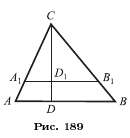
\includegraphics{mppics/ris-189}
\caption{}\label{1938/ris-189}
\end{wrapfigure}

Удобнее всего выбрать центр подобия прямо в точке $C$.
В таком случае построение искомого треугольника становится особенно простым (рис.~\ref{1938/ris-189}).
Продолжаем высоту $CD_1$ треугольника $A_1B_1C$, откладываем на ней отрезок $CD$, равный $h$, и проводим прямую $AB$, параллельную $A_1B_1$.
Треугольник $ABC$ — искомый. 

\medskip

В задачах этого рода положение искомой фигуры остаётся произвольным;
но во многих вопросах требуется построить фигуру, положение которой относительно данных точек или линий вполне определено.
При этом может случиться, что, отрешившись от какого-нибудь одного из условий положения и оставив все остальные, мы получим бесчисленное множество фигур, \so{подобных} искомой.
В таком случае метод подобия может быть употреблён с пользой.
Приведём примеры.

\smallskip
\so{Задача 2}.
\emph{В данный угол $ABC$ вписать окружность, которая проходила бы через данную точку $M$} (рис.~\ref{1938/ris-190}).

\begin{figure}[h]
\centering
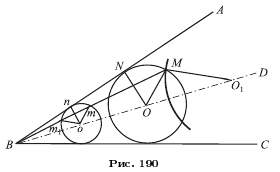
\includegraphics{mppics/ris-190}
\caption{}\label{1938/ris-190}
\end{figure}

Отбросим на время требование, чтобы окружность проходила через точку $M$.
Тогда данному условию удовлетворяет бесчисленное множество окружностей, центры которых лежат на биссектрисе $BD$.
Построим одну из таких окружностей; обозначим её центр буквой $o$. 
Возьмём на ней точку $m$, соответственную точке $M$, то есть лежащую на луче $MB$, и проведём радиус $mo$.
Если построим $MO\parallel mo$, то точка $O$ будет центром искомого круга.
Действительно, проведя к стороне $AB$ перпендикуляры $ON$ и $on$, мы получим подобные треугольники $MBO$ и $mBo$, $NBO$ и $nBo$, из которых будем иметь:
\[\frac{MO}{mo} = \frac{BO}{Bo}, \quad 
 \frac{NO}{no} = \frac{BO}{Bo},
\]
откуда 
\[\frac{MO}{mo} = \frac{NO}{no}.\]
Но $mo =no$;
следовательно, $MO=NO$, то есть окружность, описанная радиусом $OM$ с центром $O$, касается стороны $AB$;
а так как её центр лежит на биссектрисе угла, то она касается и стороны $BC$.

За соответственную точку можно взять и другую точку $m_1$ пересечения окружности с лучом $MB$.
Так мы найдём другой центр $O_1$ искомого круга.
Следовательно, задача допускает два решения.

\medskip

\begin{wrapfigure}{r}{40mm}
\vskip-5mm
\centering
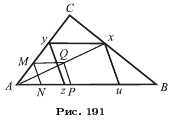
\includegraphics{mppics/ris-191}
\caption{}\label{1938/ris-191}
\end{wrapfigure}

\mbox{\so{Задача 3}.}
\emph{В данный треугольник $ABC$ вписать ромб с данным острым углом так, чтобы одна из его сторон лежала на основании $AB$ треугольника $ABC$, а две его вершины — на боковых сторонах $AC$ и $BC$} (рис.~\ref{1938/ris-191}).

Отбросим на время требование, чтобы одна из вершин ромба лежала на стороне $BC$.
Тогда можно построить бесчисленное множество ромбов, удовлетворяющих остальным условиям задачи.
Построим один из них.

Берём на стороне $AC$ произвольную точку $M$.
Строим угол с вершиной в этой точке, равный данному, одна сторона которого была бы параллельна основанию $AB$, а другая пересекала основание $AB$ в некоторой точке $N$.
На стороне $AB$ от точки $N$ откладываем отрезок $NP$, равный $MN$, и строим ромб со сторонами $MN$ и $NP$.

Пусть $Q$ — его четвёртая вершина.
Далее, выбираем вершину $A$ за центр подобия и строим ромб, подобный ромбу $MNPQ$, выбирая коэффициент подобия так, чтобы вершина нового ромба, соответствующая вершине $Q$, оказалась на стороне $BC$.
Для этой цели продолжаем прямую $AQ$ до пересечения со стороной $BC$ в некоторой точке $x$.
Эта точка $x$ будет одной из вершин искомого ромба.

Проводя из этой точки прямые, параллельные сторонам ромба $MNPQ$, получаем искомый ромб $xyzu$.

Предоставляем самим учащимся решить методом подобия следующие задачи:

1.
Построить треугольник, зная два его угла и радиус описанной окружности.

2.
Построить треугольник, зная отношение высоты к основанию, угол при вершине и медиану боковой стороны.

3.
Дан $\angle AOB$ и внутри него точка $C$.
Найти на стороне $OB$ точку $M$, равно отстоящую от $OA$ и от точки $C$.
